\chapter{Soluzione proposta}
\label{SoluzioneProposta}
\thispagestyle{empty}

\vspace{0.5cm}

\noindent In questo capitolo descriviamo la soluzione che abbiamo proposto per risolvere il problema del tampering detection, formulato nel capitolo \ref{FormulazioneProblema}.
\section{Indicatori utilizzati per identificare gli eventi di tampering}
\subsection{Misura della sfocatura nell'immagine}
Nel paragrafo \ref{sfocatura} abbiamo modellizzato il fenomeno della sfocatura secondo la formula \eqref{blur_multi}:
\[z_i(x)=\mathcal{D}_i[y_i](x) = \mathcal{B}_i[y_i](x) + \eta(x), \qquad x \in \mathcal{X}.\]
Ricavare un indicatore in grado di misurare direttamente il grado di sfocatura di un'immagine \`e difficile.
Quello che \`e possibile fare, come proposto in \cite{alippi2010detecting}, \`e utilizzare una misura \textit{indiretta} di questo operatore.\\
Come abbiamo visto nel paragrafo \ref{sfocatura}, l'operatore di sfocatura $\mathcal{B}$ ha come effetto principale quello di rendere le differenze di intensit\`a tra pixel adiacenti pi\`u morbide (\textit{smooth}).
In base a questo \`e possibile identificare un evento di sfocatura andando a monitorare l'\textit{energia media del gradiente} di ciascuna immagine:
\begin{equation}
\label{eq:energyGradient}
g_i = \mathcal{G}[z_i] =\frac{\sum_{\mathcal{X}}\| \nabla z_i(x) \| _2^2 }{|\mathcal{X}|} ,
\end{equation}  
dove abbiamo indicato con $|\mathcal{X}|$ la \textit{cardinalit\`a} dell'insieme dei pixel $\mathcal{X}$, e con $\|\cdot\|_2$ la norma di tipo $\mathcal{L}_2$\footnote{$\|x\|_2=\sqrt{\sum_{i}x_i^2}$}.\\
Lavorando nel dominio discreto delle immagini digitali, possiamo calcolare le derivate dell'intensit\`a luminosa (\textit{luma}) per mezzo di convoluzioni con filtri derivativi.
In particolare, per il calcolo delle derivate orizzontali  abbiamo utilizzato il seguente filtro $f_i$:
\[f_i = f \circledast \left[ \begin{array}{rcl}
1 & 0 & -1
\end{array}\right], \] 
mentre per il calcolo delle derivate verticali  abbiamo utilizzato il seguente filtro $f_j$:
\[f_j = f \circledast \left[ \begin{array}{r}
1 \\ 0 \\ -1
\end{array}\right], \]
dove abbiamo indicato con $\circledast$ l'operatore di convoluzione e con $f$ un \textit{filtro gaussiano} di dimensione $5 \times 5$:
\[f(i,j)=\frac{1}{2\pi\sigma^2}\exp\left(-\frac{\left(i-k-1\right)^2+\left(j-k-1\right)^2}{2\sigma^2}\right)\] 
dove $k=2$ e  la deviazione standard $\sigma = 1$.
Con questi filtri \`e possibile calcolare la \textit{norma del gradiente} nel seguente modo:
\[\| \nabla z_i(x) \|_2^2=\left(z \circledast f_i\right)(x)^2 + \left(z \circledast f_j\right)(x)^2.\]
Una volta calcolata la norma del gradiente \`e possibile farne la media come specificato nella formula \eqref{eq:energyGradient}.
Il risultato finale \`e un indicatore \textit{scalare} per ciascun frame acquisito, che pu\`o essere monitorato per individuare eventi di sfocature. 
In particolare l'evento \`e associato a un \textit{crollo} del valore di $g$.
\subsection{Misura del displacement}
Nel paragrafo \ref{displacement} abbiamo modellizzato il fenomeno dello spostamento della camera secondo la formula \eqref{eq:displacement}
\[z_i(x)  = \left\{ \begin{array}{rcl}
y_i(x) + \eta(x) & \mbox{per} & i < T^* \\
w_i(x) + \eta(x) & \mbox{per} & i \geqslant T^*
\end{array}\right. , x \in \mathcal{X}\]
dove $T^*$ indica l'istante in cui avviene il cambiamento.\\
Uno spostamento della camera, quindi, \`e associato a un cambiamento \textit{globale} dei valori di intensit\`a luminosa (\textit{luma}) nei pixel dell'immagine.
In base a questo \`e possibile identificare un evento di spostamento della camera andando a monitorare l'\textit{energia media della luma} di ciascuna immagine:
\begin{equation}
\label{eq:energyLuma}
l_i = \mathcal{L}[z_i] =\frac{\sum_{\mathcal{X}} z_i(x) }{|\mathcal{X}|} ,
\end{equation}  
dove abbiamo indicato con $|\mathcal{X}|$ la \textit{cardinalit\`a} dell'insieme dei pixel $\mathcal{X}$.\\
Il risultato finale \`e un indicatore \textit{scalare} per ciascun frame acquisito, che pu\`o essere monitorato per individuare eventi di spostamenti della camera. 
\subsection{Comportamento degli indicatori nel tempo}
Analizzando alcune sequenze video abbiamo notato che, anche in assenza di eventi di tampering, vi sono alcuni fattori che sono in grado di far variare il valore degli indicatori estratti.
Tra i pi\`u importanti abbiamo:
\begin{itemize}
	\item \textit{Cambi di luminosit\`a} che avvengono nel corso della giornata. 
	Se consideriamo l'esempio in figura \ref{fig:testiGN}, possiamo notare come, nel passaggio dal giorno (figura \ref{fig:FTgiorno}) alla notte (figura \ref{fig:FTnotte}), le differenze di luminosit\`a siano elevate.  
%	
%	Considerando acquisizioni fatte all'esterno, il caso pi\`u evidente avviene durante il \textit{passaggio dal giorno alla notte}, come possiamo vedere ad esempio la variazione che abbiamo tra il frame in figura \ref{fig:FTgiorno} e il frame in figura \ref{fig:FTnotte}.
	\item \textit{Dinamicit\`a della scena}. La ripresa di una scena movimentata, come ad esempio una strada, ha come risultato che ciascun frame sia diverso dagli altri.
	Ci\`o si traduce in una variabilit\`a elevata degli indicatori che abbiamo utilizzato. 
	Inoltre, col passare del tempo, pu\`o succedere che cambi anche il \textit{grado di dinamicit\`a} della scena.
	Considerando ancora l'esempio della strada, infatti, avremo dei momenti in cui il traffico \`e pi\`u intenso (nelle cosiddette \textit{ore di punta}) e altri in cui le macchine passano meno spesso (tipicamente durante la notte).
	\item \textit{Configurazione automatica della camera}. Solitamente le camere sono in grado di configurare in maniera automatica alcuni parametri, in base alle condizioni di luminosit\`a esterne.
	Ad esempio, durante la ripresa di scene notturne la camera solitamente aumenta il \textit{tempo di esposizione} del sensore, in modo da ricevere pi\`u luce possibile.
	Ci\`o si traduce in un \textit{aumento del rumore} su tutta la scena acquisita (come vediamo nel frame in figura \ref{fig:FTnotte}) e in una \textit{presenza di sfocature} quando vengono immortalati degli oggetti in movimento (come ad esempio le macchine che si muovono nella figura \ref{fig:BAnotte}).
\end{itemize} 
\begin{figure}
	\centering
	\begin{subfigure}[]
		{\label{fig:FTgiorno} 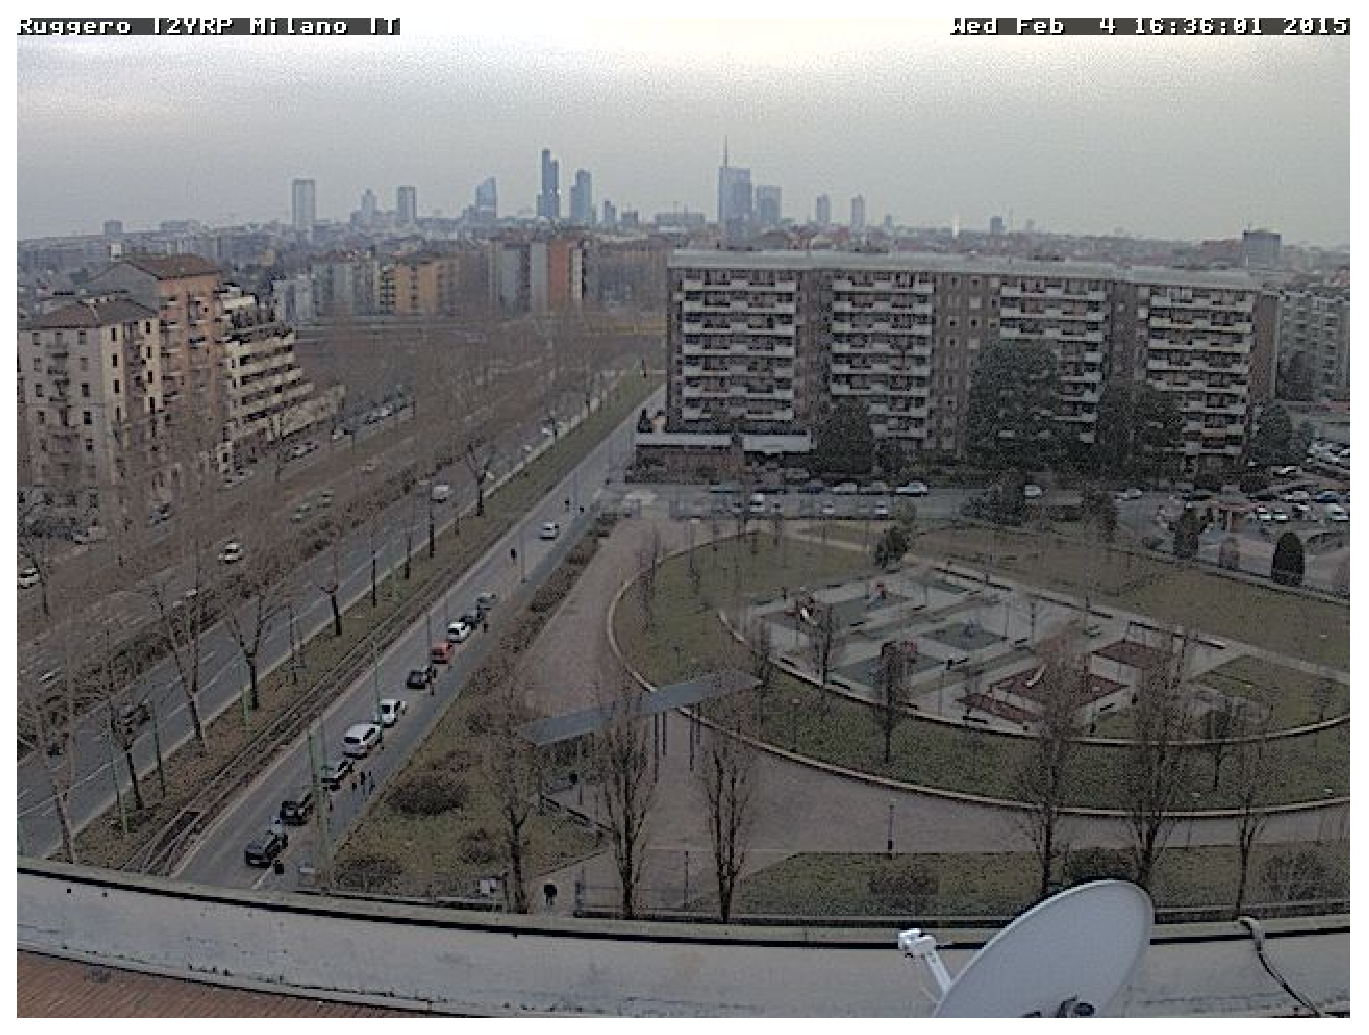
\includegraphics[width=6cm]{./pictures/testiGIORNO}}
	\end{subfigure}
	\begin{subfigure}[]
		{\label{fig:FTnotte} 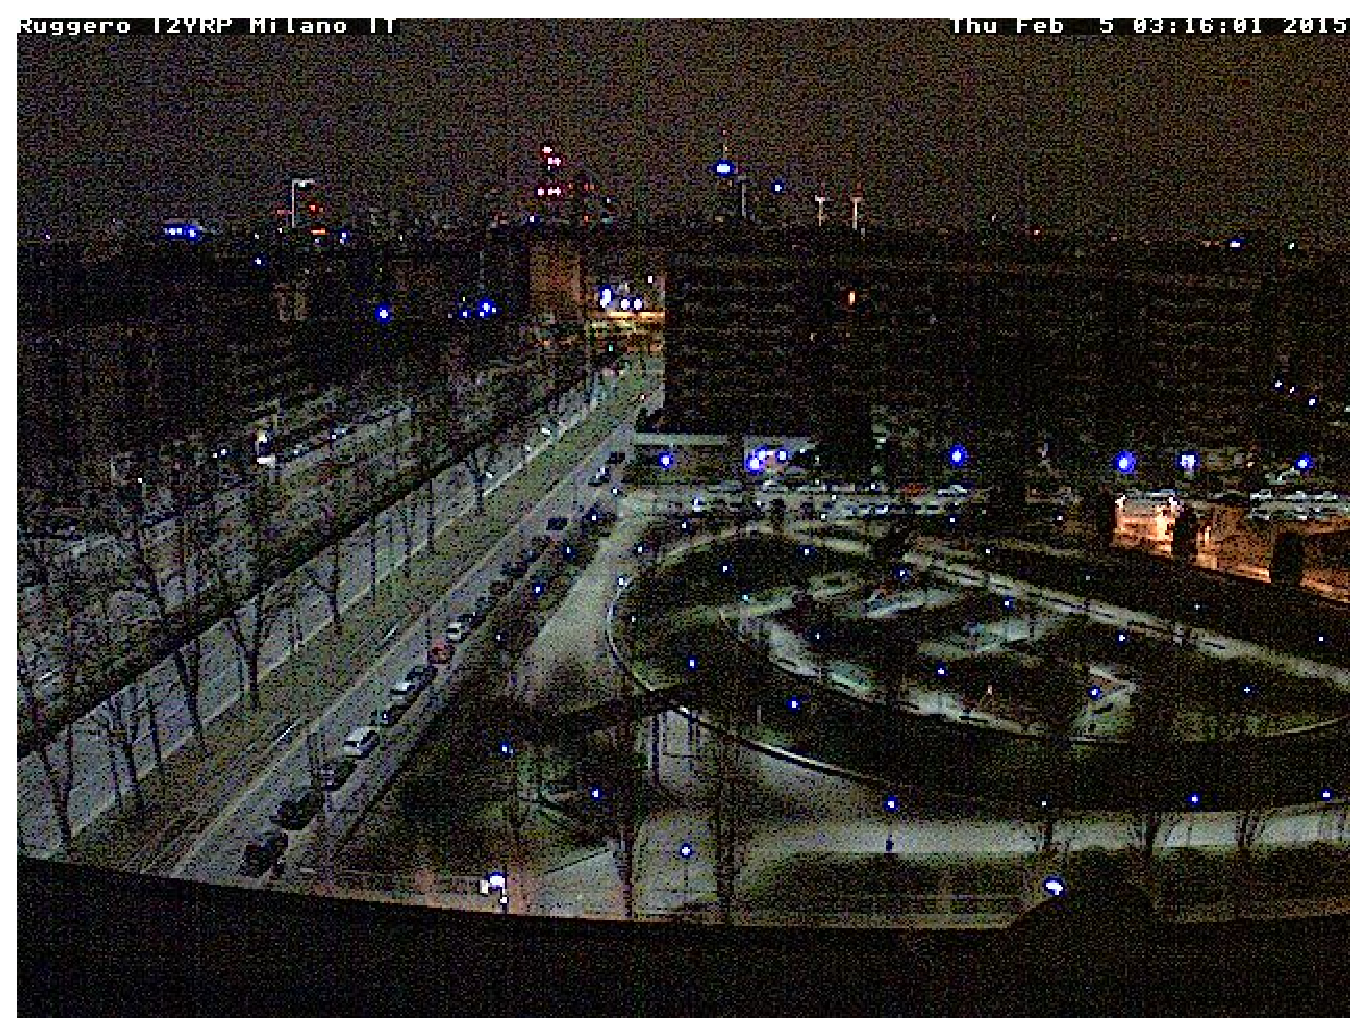
\includegraphics[width=6cm]{./pictures/testiNOTTE}}
	\end{subfigure}
	\caption{Esempio di cambi di luminosit\`a tra il giorno e la notte}
	\label{fig:testiGN}
\end{figure}
\begin{figure}
	\centering
	\begin{subfigure}[]
		{\label{fig:BAgiorno} 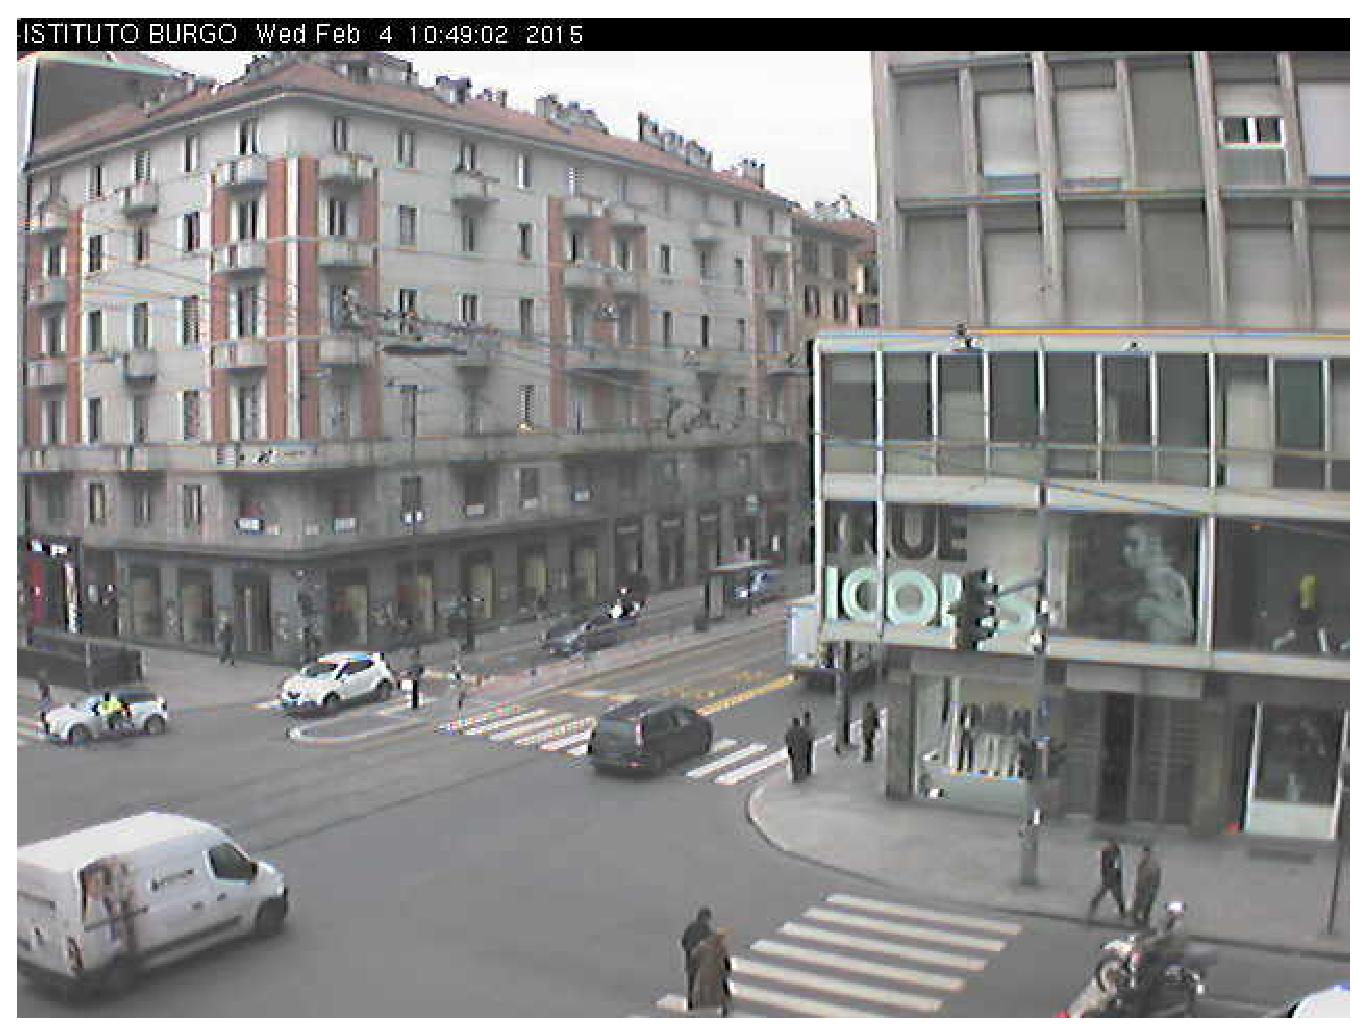
\includegraphics[width=6cm]{./pictures/buenosAiresGIORNO}}
	\end{subfigure}
	\begin{subfigure}[]
		{\label{fig:BAnotte} 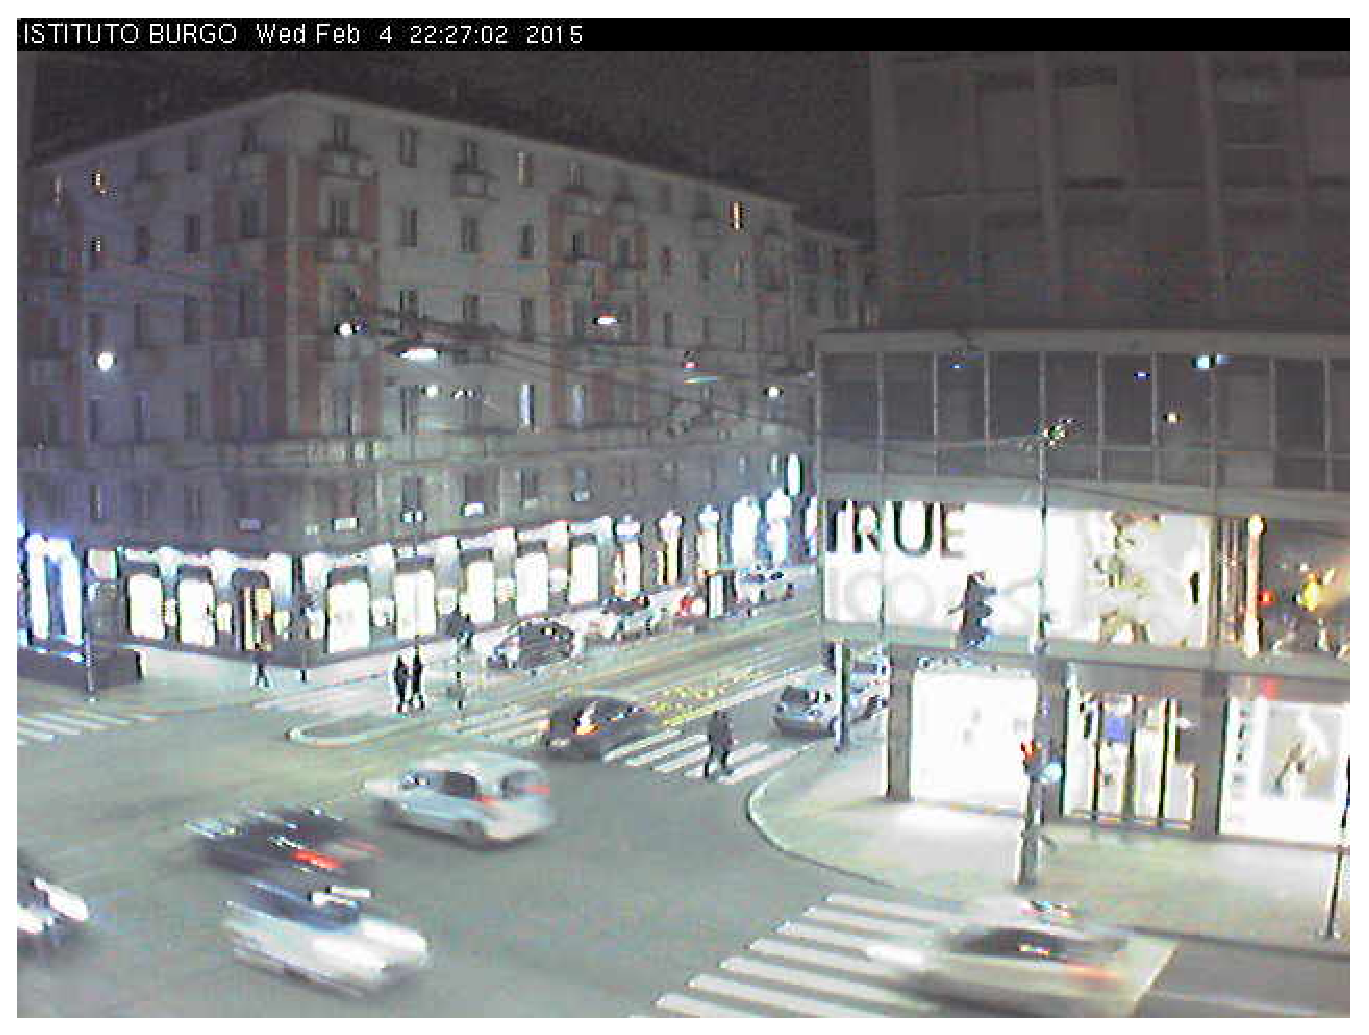
\includegraphics[width=6cm]{./pictures/buenosAiresNOTTE}}
	\end{subfigure}
	\caption{Esempio di presenza di sfocature dovute all'aumento del tempo di esposizione della camera}
	\label{fig:buenosAiresGN}
\end{figure}
Questi fenomeni fanno s\`i che i nostri indicatori abbiano una dinamica \textit{difficilmente prevedibile} e che \textit{non siano stazionari}, come possiamo vedere negli esempi delle figure \ref{fig:energy} e \ref{fig:luma}.
\begin{figure}
\centering
\begin{subfigure}[]
	{\label{fig:energy} 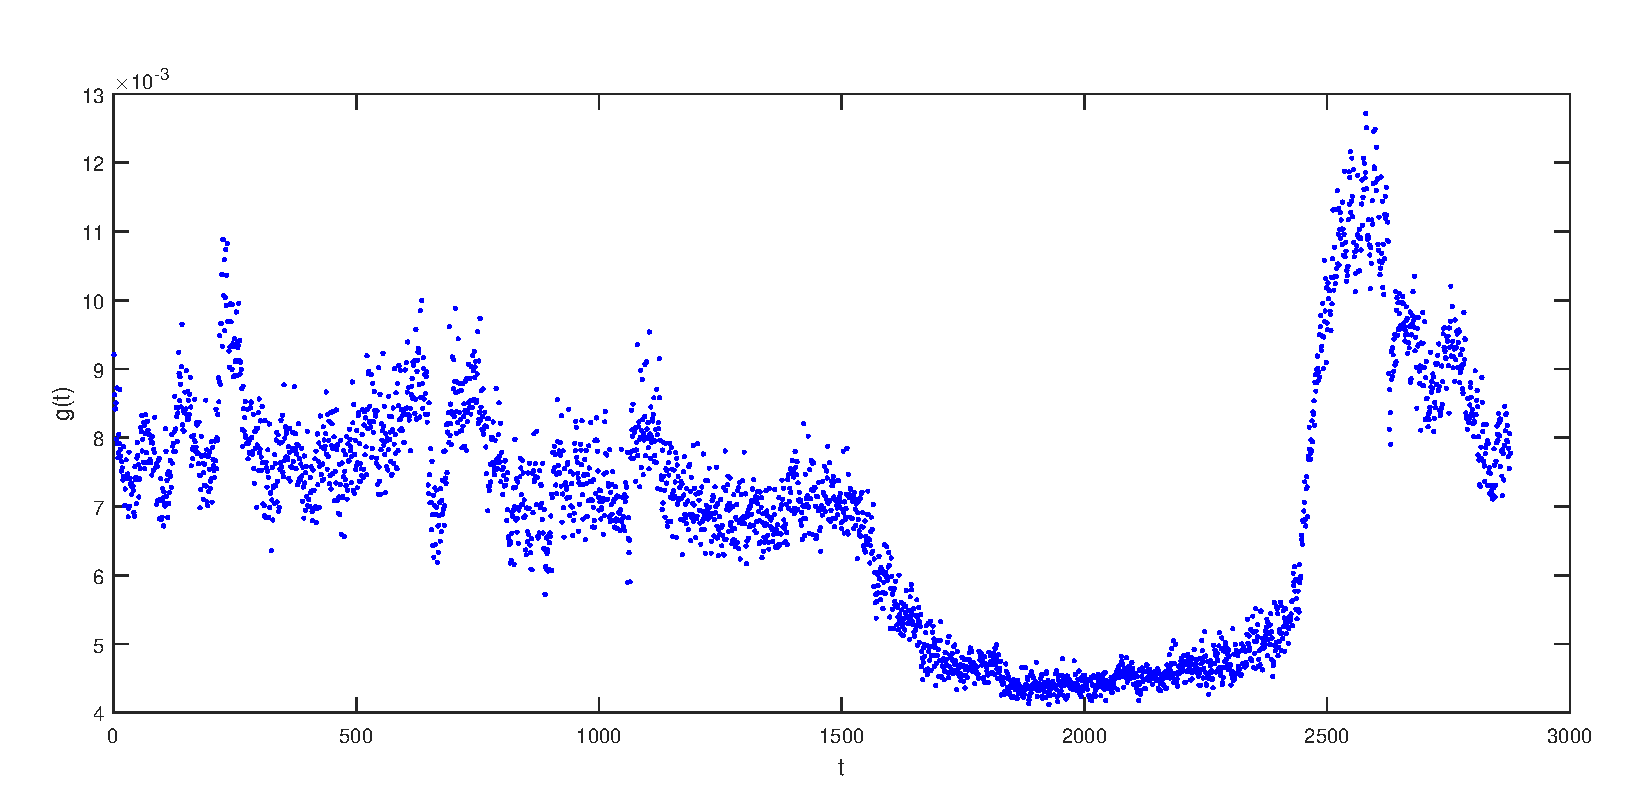
\includegraphics[width=13cm]{./pictures/energyTot}}
\end{subfigure}
\begin{subfigure}[]
	{\label{fig:energyDetr} 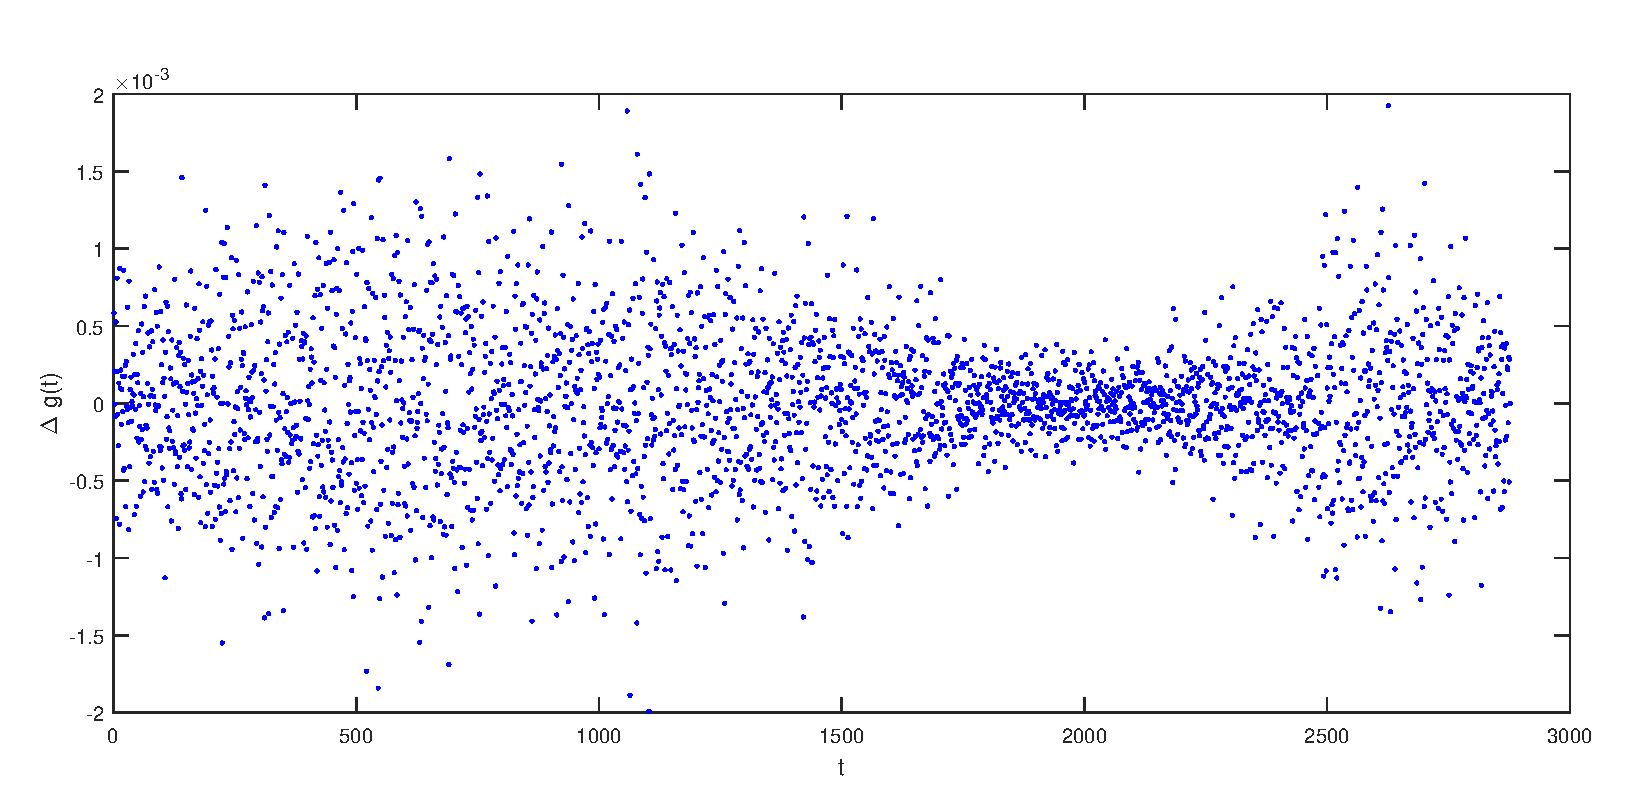
\includegraphics[width=13cm]{./pictures/energydetr}}
\end{subfigure}
\caption{Energia media del gradiente lungo un'acquisizione di 24 ore (a) e suo detrending (b)}
\label{fig:energyTot}
\end{figure}
\begin{figure}
	\centering
	\begin{subfigure}[]
		{\label{fig:luma} 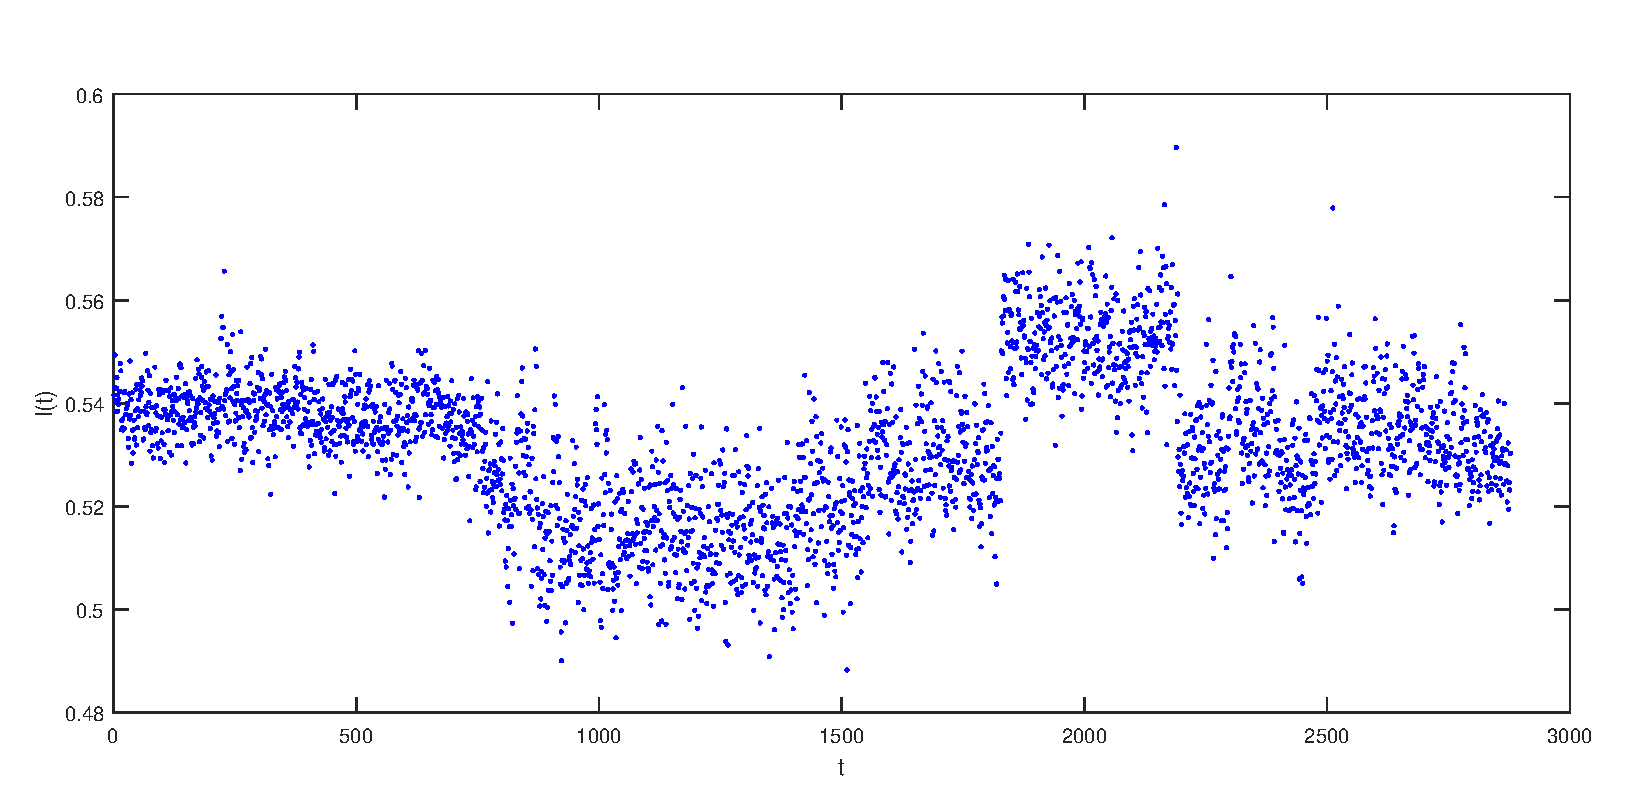
\includegraphics[width=13cm]{./pictures/lumaTot}}
	\end{subfigure}
	\begin{subfigure}[]
		{\label{fig:lumaDetr} 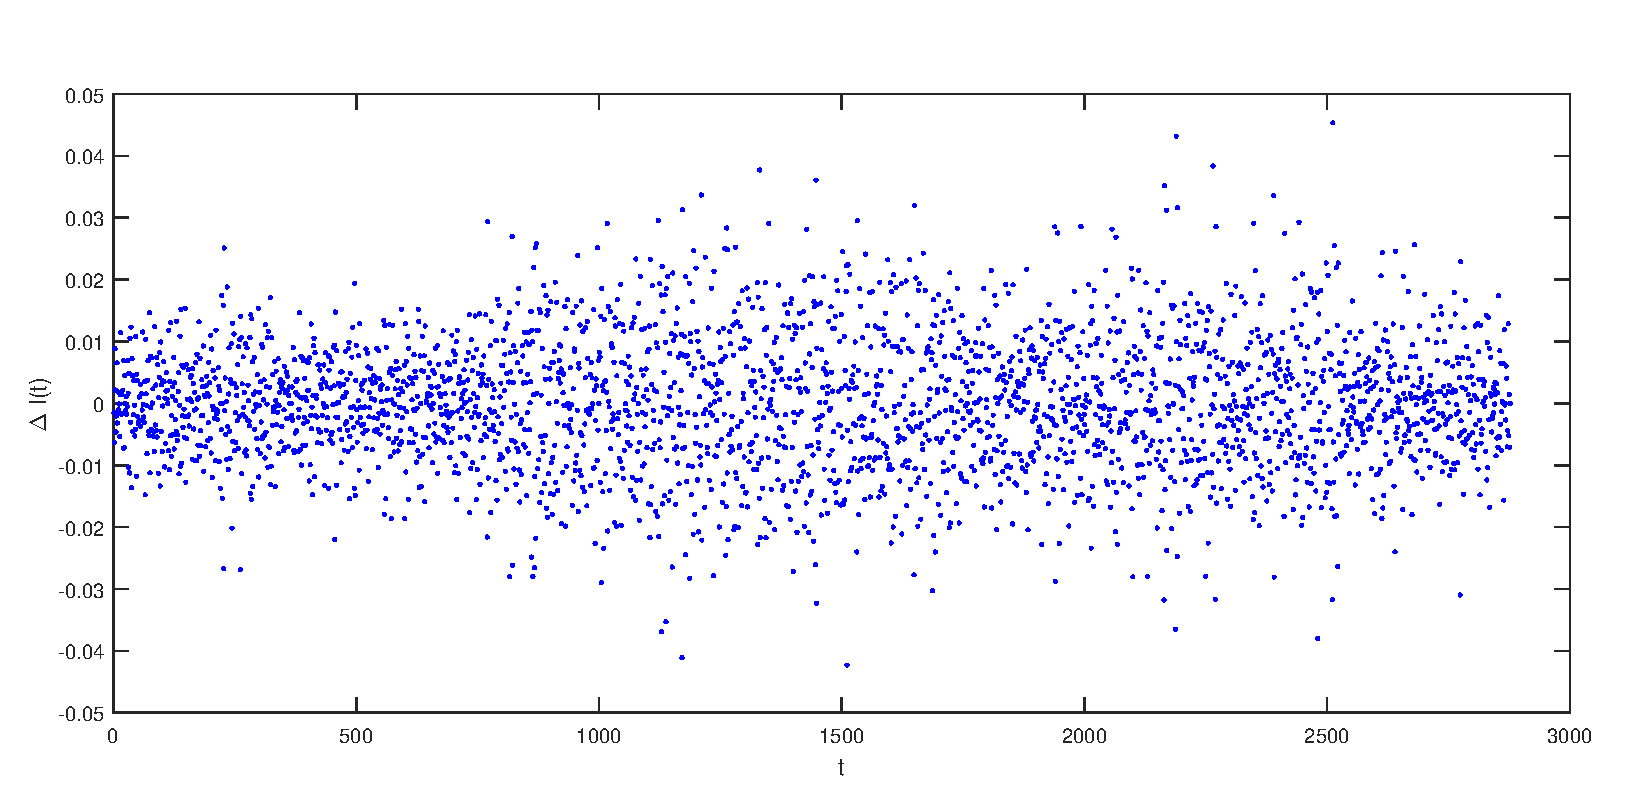
\includegraphics[width=13cm]{./pictures/lumadetr}}
	\end{subfigure}
	\caption{Energia media della luma lungo un'acquisizione di 24 ore (a) e suo detrending (b)}
	\label{fig:lumaTot}
\end{figure}
Di conseguenza non \`e possibile applicare direttamente le tecniche di CDT come fatto in \cite{alippi2010detecting}. \\
Per eliminare le componenti in bassa frequenza possiamo fare un \textit{detrending} sulle sequenze facendo una convoluzione con un \textit{filtro derivativo}
\[df=\left[\begin{array}{rl}
-1 & 1
\end{array}\right].\]
Il comportamento del detrending sulle sequenze degli indicatori che abbiamo utilizzato \`e rappresentato nelle figure \ref{fig:energyDetr} e \ref{fig:lumaDetr}.  
\section{Tecniche di monitoraggio degli indicatori}
\subsection{Monitoraggio one-shot}
\subsection{Monitoraggio sequenziale}
\section{Algoritmo di segmentazione}
